\documentclass[a4paper]{report}
\usepackage{graphicx}
\usepackage{xspace,ifthen,epsfig}
\usepackage{cite}
\usepackage{color}
\usepackage{fancybox}
\usepackage{float}
\usepackage{subfigure}
\usepackage{longtable} 
\usepackage{tabularx} 
\usepackage{ltxtable} 
\usepackage{times}
\usepackage[table]{xcolor}
\usepackage{url}
\usepackage{listings}
\usepackage{amsmath}
\usepackage{dsfont}
\usepackage[american]{babel}
\usepackage[utf8]{inputenc}
\usepackage{fancyhdr}
\usepackage{booktabs}
\usepackage{tikz,pgfplots}
\usepackage{todonotes}
\usepackage{footmisc}
\usepackage{marvosym}
\usepackage{hyperref}

\usetikzlibrary{pgfplots.statistics}
\pgfplotsset{
  width=60mm,height=55mm,
  major grid style={thin,dotted,color=black!50},
  minor grid style={thin,dotted,color=black!50},
  grid,
  every axis/.append style={
    line width=0.5pt,
    tick style={
      line cap=round,
      thin,
      major tick length=4pt,
      minor tick length=2pt,
    },
  },
  /pgf/number format/1000 sep={},
  legend cell align=left,
  legend pos=north west,
  log y ticks with fixed point/.style={
      yticklabel={
        \pgfkeys{/pgf/fpu=true}
        \pgfmathparse{exp(\tick)}%
        \pgfmathprintnumber[fixed relative, precision=3]{\pgfmathresult}
        \pgfkeys{/pgf/fpu=false}
      }
  },
}

\begin{document}

\begin{figure}[H]
    % IMPORT-DATA urls data/uk-2007-05.urls.txt
    \centering
    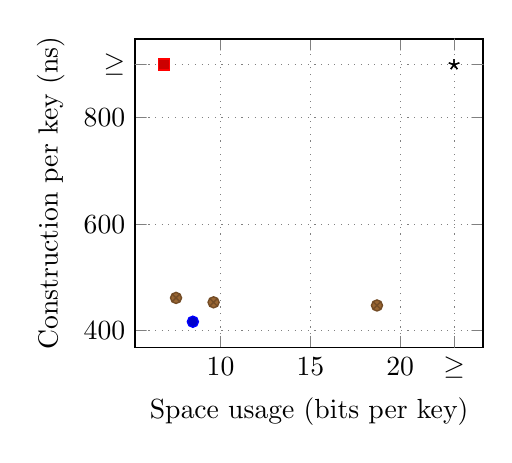
\begin{tikzpicture}
        \begin{axis}[
            title={},
            xlabel={Space usage (bits per key)},
            ylabel={Construction per key (ns)},
            legend style={at={(1.03,0.5)},anchor=west},
            legend columns=4,
            only marks,
            extra x ticks={23},
            extra x tick labels={$\geq$},
            extra y ticks={900},
            extra y tick labels={$\geq$},
            legend to name=legendUrls,
          ]
          %% MULTIPLOT(name|title)
          %%   SELECT
          %%     MIN(bitsPerElement, 23) as x,
          %%     MIN(1000000.0*constructionTimeMilliseconds/N, 900) as y,
          %%     name,
          %%     name AS title
          %%   FROM urls
          %%   ORDER BY name,x
          \addplot coordinates { (8.45766,416.5) };
          \addlegendentry{CentroidHollowTrie};
          \addplot coordinates { (6.85742,900) };
          \addlegendentry{DirectRankStoring};
          \addplot coordinates { (7.52016,461.3) (9.61119,453.0) (18.7085,447.1) };
          \addlegendentry{HollowTrie};
          \addplot coordinates { (23,900) (23,900) };
          \addlegendentry{PathDecomposedTrie};
        \end{axis}
    \end{tikzpicture}
    \hfill
    \begin{tikzpicture}
        \begin{axis}[
            title={},
            xlabel={Space usage (bits per key)},
            ylabel={Query time ($\mu$s)},
            only marks,
            extra x ticks={23},
            extra x tick labels={$\geq$},
            extra y ticks={900},
            extra y tick labels={$\geq$},
          ]
          %% MULTIPLOT(name|title)
          %%   SELECT
          %%     MIN(bitsPerElement, 23) as x,
          %%     1000.0*queryTimeMilliseconds/numQueries as y,
          %%     name,
          %%     name AS title
          %%   FROM urls
          %%   ORDER BY name,x
          \addplot coordinates { (8.45766,1.77) };
          \addlegendentry{CentroidHollowTrie};
          \addplot coordinates { (6.85742,3.5) };
          \addlegendentry{DirectRankStoring};
          \addplot coordinates { (7.52016,4.78) (9.61119,4.88) (18.7085,3.18) };
          \addlegendentry{HollowTrie};
          \addplot coordinates { (23,3.14) (23,3.51) };
          \addlegendentry{PathDecomposedTrie};

          \legend{};
        \end{axis}
    \end{tikzpicture}

    \caption{Measurements on the \texttt{uk-2007-05.urls} data set.}
\end{figure}

\begin{figure}[H]
    % IMPORT-DATA titles data/trec-title.terms.txt
    \centering
    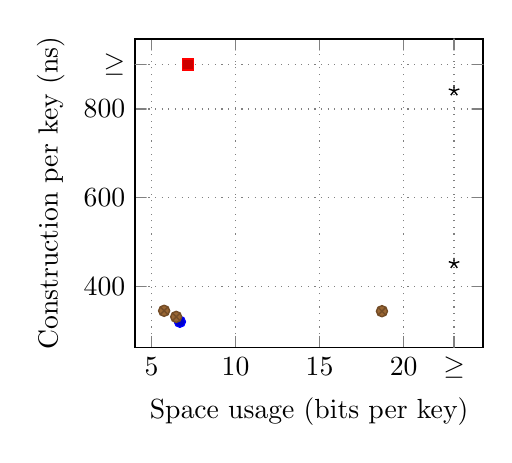
\begin{tikzpicture}
        \begin{axis}[
            title={},
            xlabel={Space usage (bits per key)},
            ylabel={Construction per key (ns)},
            legend style={at={(1.03,0.5)},anchor=west},
            legend columns=4,
            only marks,
            extra x ticks={23},
            extra x tick labels={$\geq$},
            extra y ticks={900},
            extra y tick labels={$\geq$},
          ]
          %% MULTIPLOT(name|title)
          %%   SELECT
          %%     MIN(bitsPerElement, 23) as x,
          %%     MIN(1000000.0*constructionTimeMilliseconds/N, 900) as y,
          %%     name,
          %%     name AS title
          %%   FROM titles
          %%   ORDER BY name,x
          \addplot coordinates { (6.69053,321.177) };
          \addlegendentry{CentroidHollowTrie};
          \addplot coordinates { (7.1703,900) };
          \addlegendentry{DirectRankStoring};
          \addplot coordinates { (5.75304,345.813) (6.4705,332.126) (18.7111,344.9) };
          \addlegendentry{HollowTrie};
          \addplot coordinates { (23,452.568) (23,841.265) };
          \addlegendentry{PathDecomposedTrie};

          \legend{};
        \end{axis}
    \end{tikzpicture}
    \hfill
    \begin{tikzpicture}
        \begin{axis}[
            title={},
            xlabel={Space usage (bits per key)},
            ylabel={Query time ($\mu$s)},
            only marks,
            extra x ticks={23},
            extra x tick labels={$\geq$},
            extra y ticks={900},
            extra y tick labels={$\geq$},
          ]
          %% MULTIPLOT(name|title)
          %%   SELECT
          %%     MIN(bitsPerElement, 23) as x,
          %%     1000.0*queryTimeMilliseconds/numQueries as y,
          %%     name,
          %%     name AS title
          %%   FROM titles
          %%   ORDER BY name,x
          \addplot coordinates { (6.69053,1.05) };
          \addlegendentry{CentroidHollowTrie};
          \addplot coordinates { (7.1703,0.63) };
          \addlegendentry{DirectRankStoring};
          \addplot coordinates { (5.75304,1.78) (6.4705,1.83) (18.7111,1.14) };
          \addlegendentry{HollowTrie};
          \addplot coordinates { (23,0.91) (23,0.9) };
          \addlegendentry{PathDecomposedTrie};

          \legend{};
        \end{axis}
    \end{tikzpicture}

    \caption{Measurements on the \texttt{trec-title.terms} data set.}
\end{figure}

\begin{figure}[H]
    % IMPORT-DATA text data/trec-text.terms.txt
    \centering
    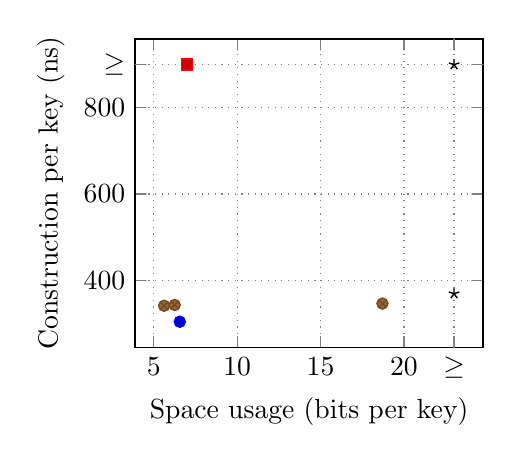
\begin{tikzpicture}
        \begin{axis}[
            title={},
            xlabel={Space usage (bits per key)},
            ylabel={Construction per key (ns)},
            legend style={at={(1.03,0.5)},anchor=west},
            legend columns=4,
            only marks,
            extra x ticks={23},
            extra x tick labels={$\geq$},
            extra y ticks={900},
            extra y tick labels={$\geq$},
          ]
          %% MULTIPLOT(name|title)
          %%   SELECT
          %%     MIN(bitsPerElement, 23) as x,
          %%     MIN(1000000.0*constructionTimeMilliseconds/N, 900) as y,
          %%     name,
          %%     name AS title
          %%   FROM text
          %%   ORDER BY name,x
          \addplot coordinates { (6.55968,303.9) };
          \addlegendentry{CentroidHollowTrie};
          \addplot coordinates { (7.00542,900) };
          \addlegendentry{DirectRankStoring};
          \addplot coordinates { (5.62218,340.9) (6.25452,342.7) (18.7085,346.0) };
          \addlegendentry{HollowTrie};
          \addplot coordinates { (23,369.0) (23,900) };
          \addlegendentry{PathDecomposedTrie};

          \legend{};
        \end{axis}
    \end{tikzpicture}
    \hfill
    \begin{tikzpicture}
        \begin{axis}[
            title={},
            xlabel={Space usage (bits per key)},
            ylabel={Query time ($\mu$s)},
            only marks,
            extra x ticks={23},
            extra x tick labels={$\geq$},
            extra y ticks={900},
            extra y tick labels={$\geq$},
          ]
          %% MULTIPLOT(name|title)
          %%   SELECT
          %%     MIN(bitsPerElement, 23) as x,
          %%     1000.0*queryTimeMilliseconds/numQueries as y,
          %%     name,
          %%     name AS title
          %%   FROM text
          %%   ORDER BY name,x
          \addplot coordinates { (6.55968,1.45) };
          \addlegendentry{CentroidHollowTrie};
          \addplot coordinates { (7.00542,0.74) };
          \addlegendentry{DirectRankStoring};
          \addplot coordinates { (5.62218,2.16) (6.25452,2.19) (18.7085,1.48) };
          \addlegendentry{HollowTrie};
          \addplot coordinates { (23,1.45) (23,1.44) };
          \addlegendentry{PathDecomposedTrie};

          \legend{};
        \end{axis}
    \end{tikzpicture}

    \begin{tikzpicture}
        \ref*{legendUrls}
    \end{tikzpicture}
    \caption{Measurements on the \texttt{trec-text.terms} data set.}
\end{figure}

\end{document}
